\begin{figure}[H]
  \centering
  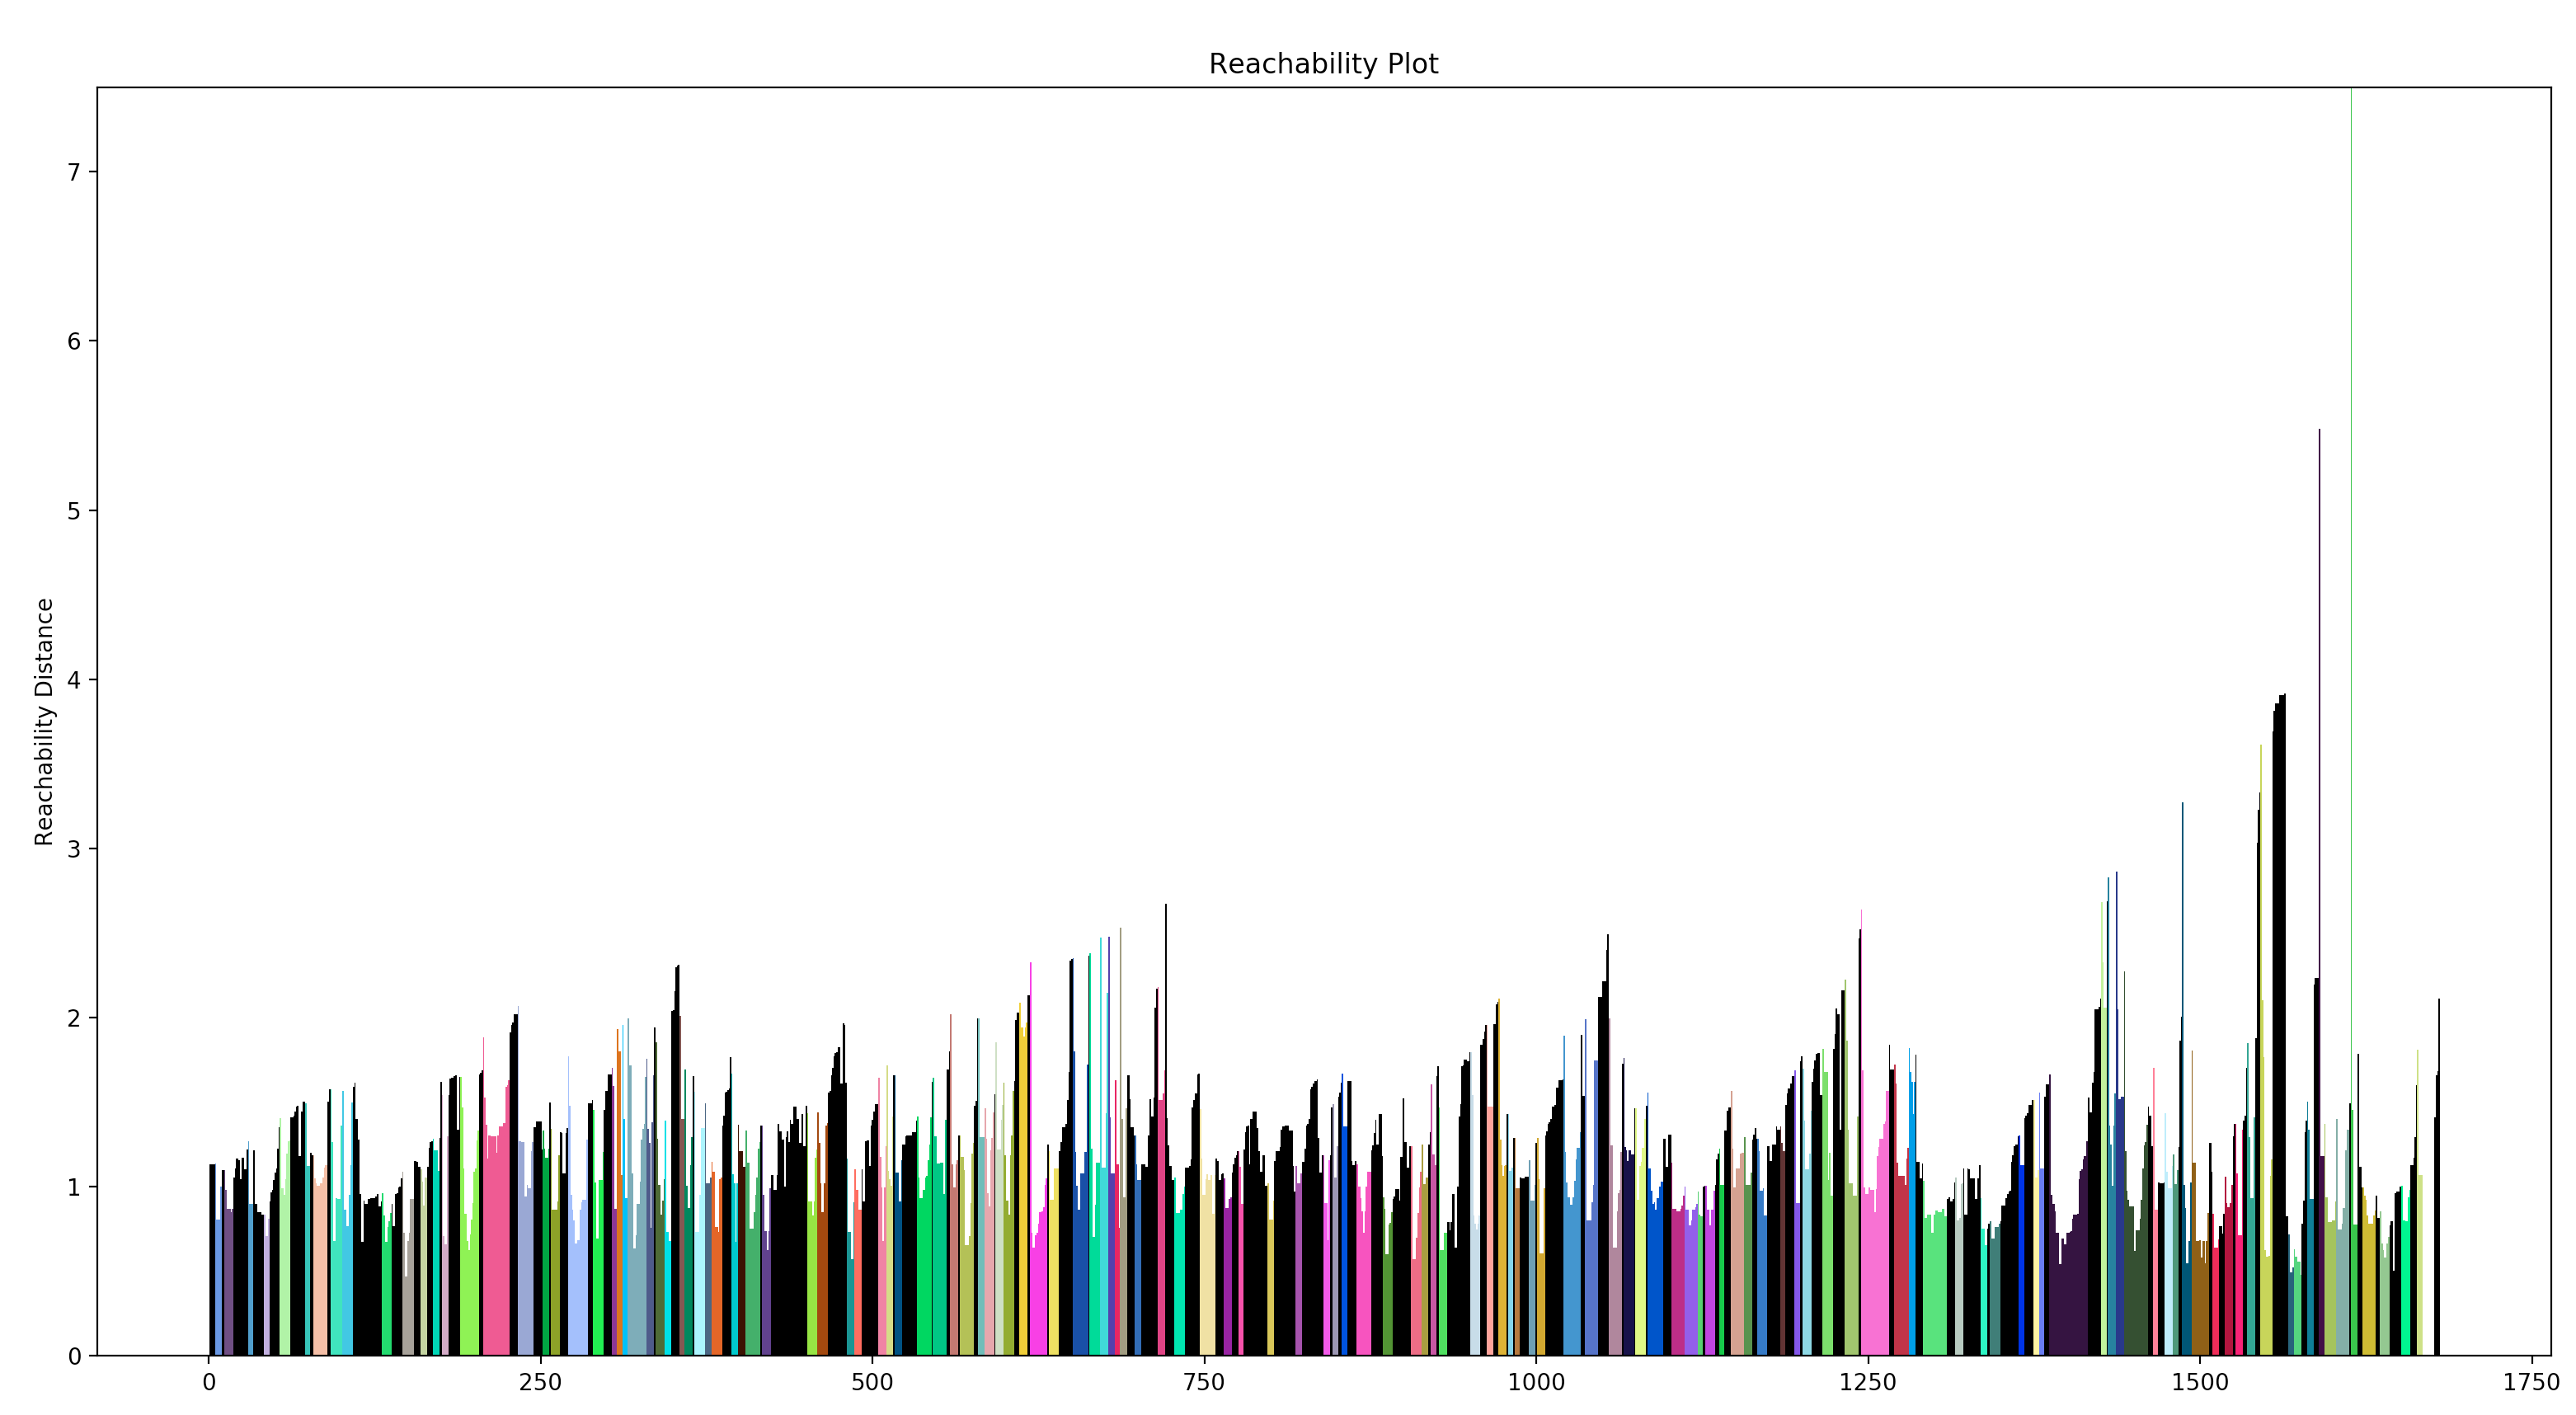
\includegraphics[width=1\textwidth]{./images/OPTICS/1h-1-reachabilityPlot-xi.png}
  \caption{\textbf{1h dataset} (first column - 15 min) OPTICS reachability plot using OPTICS automatic cluster extraction (\textbf{xi}). The coloured bars highlight clusters, whilst the black ones indicate noise.}
  \label{figure:fullSizeReachabilityPlotXi1h}
\end{figure}

\begin{figure}[H]
  \centering
  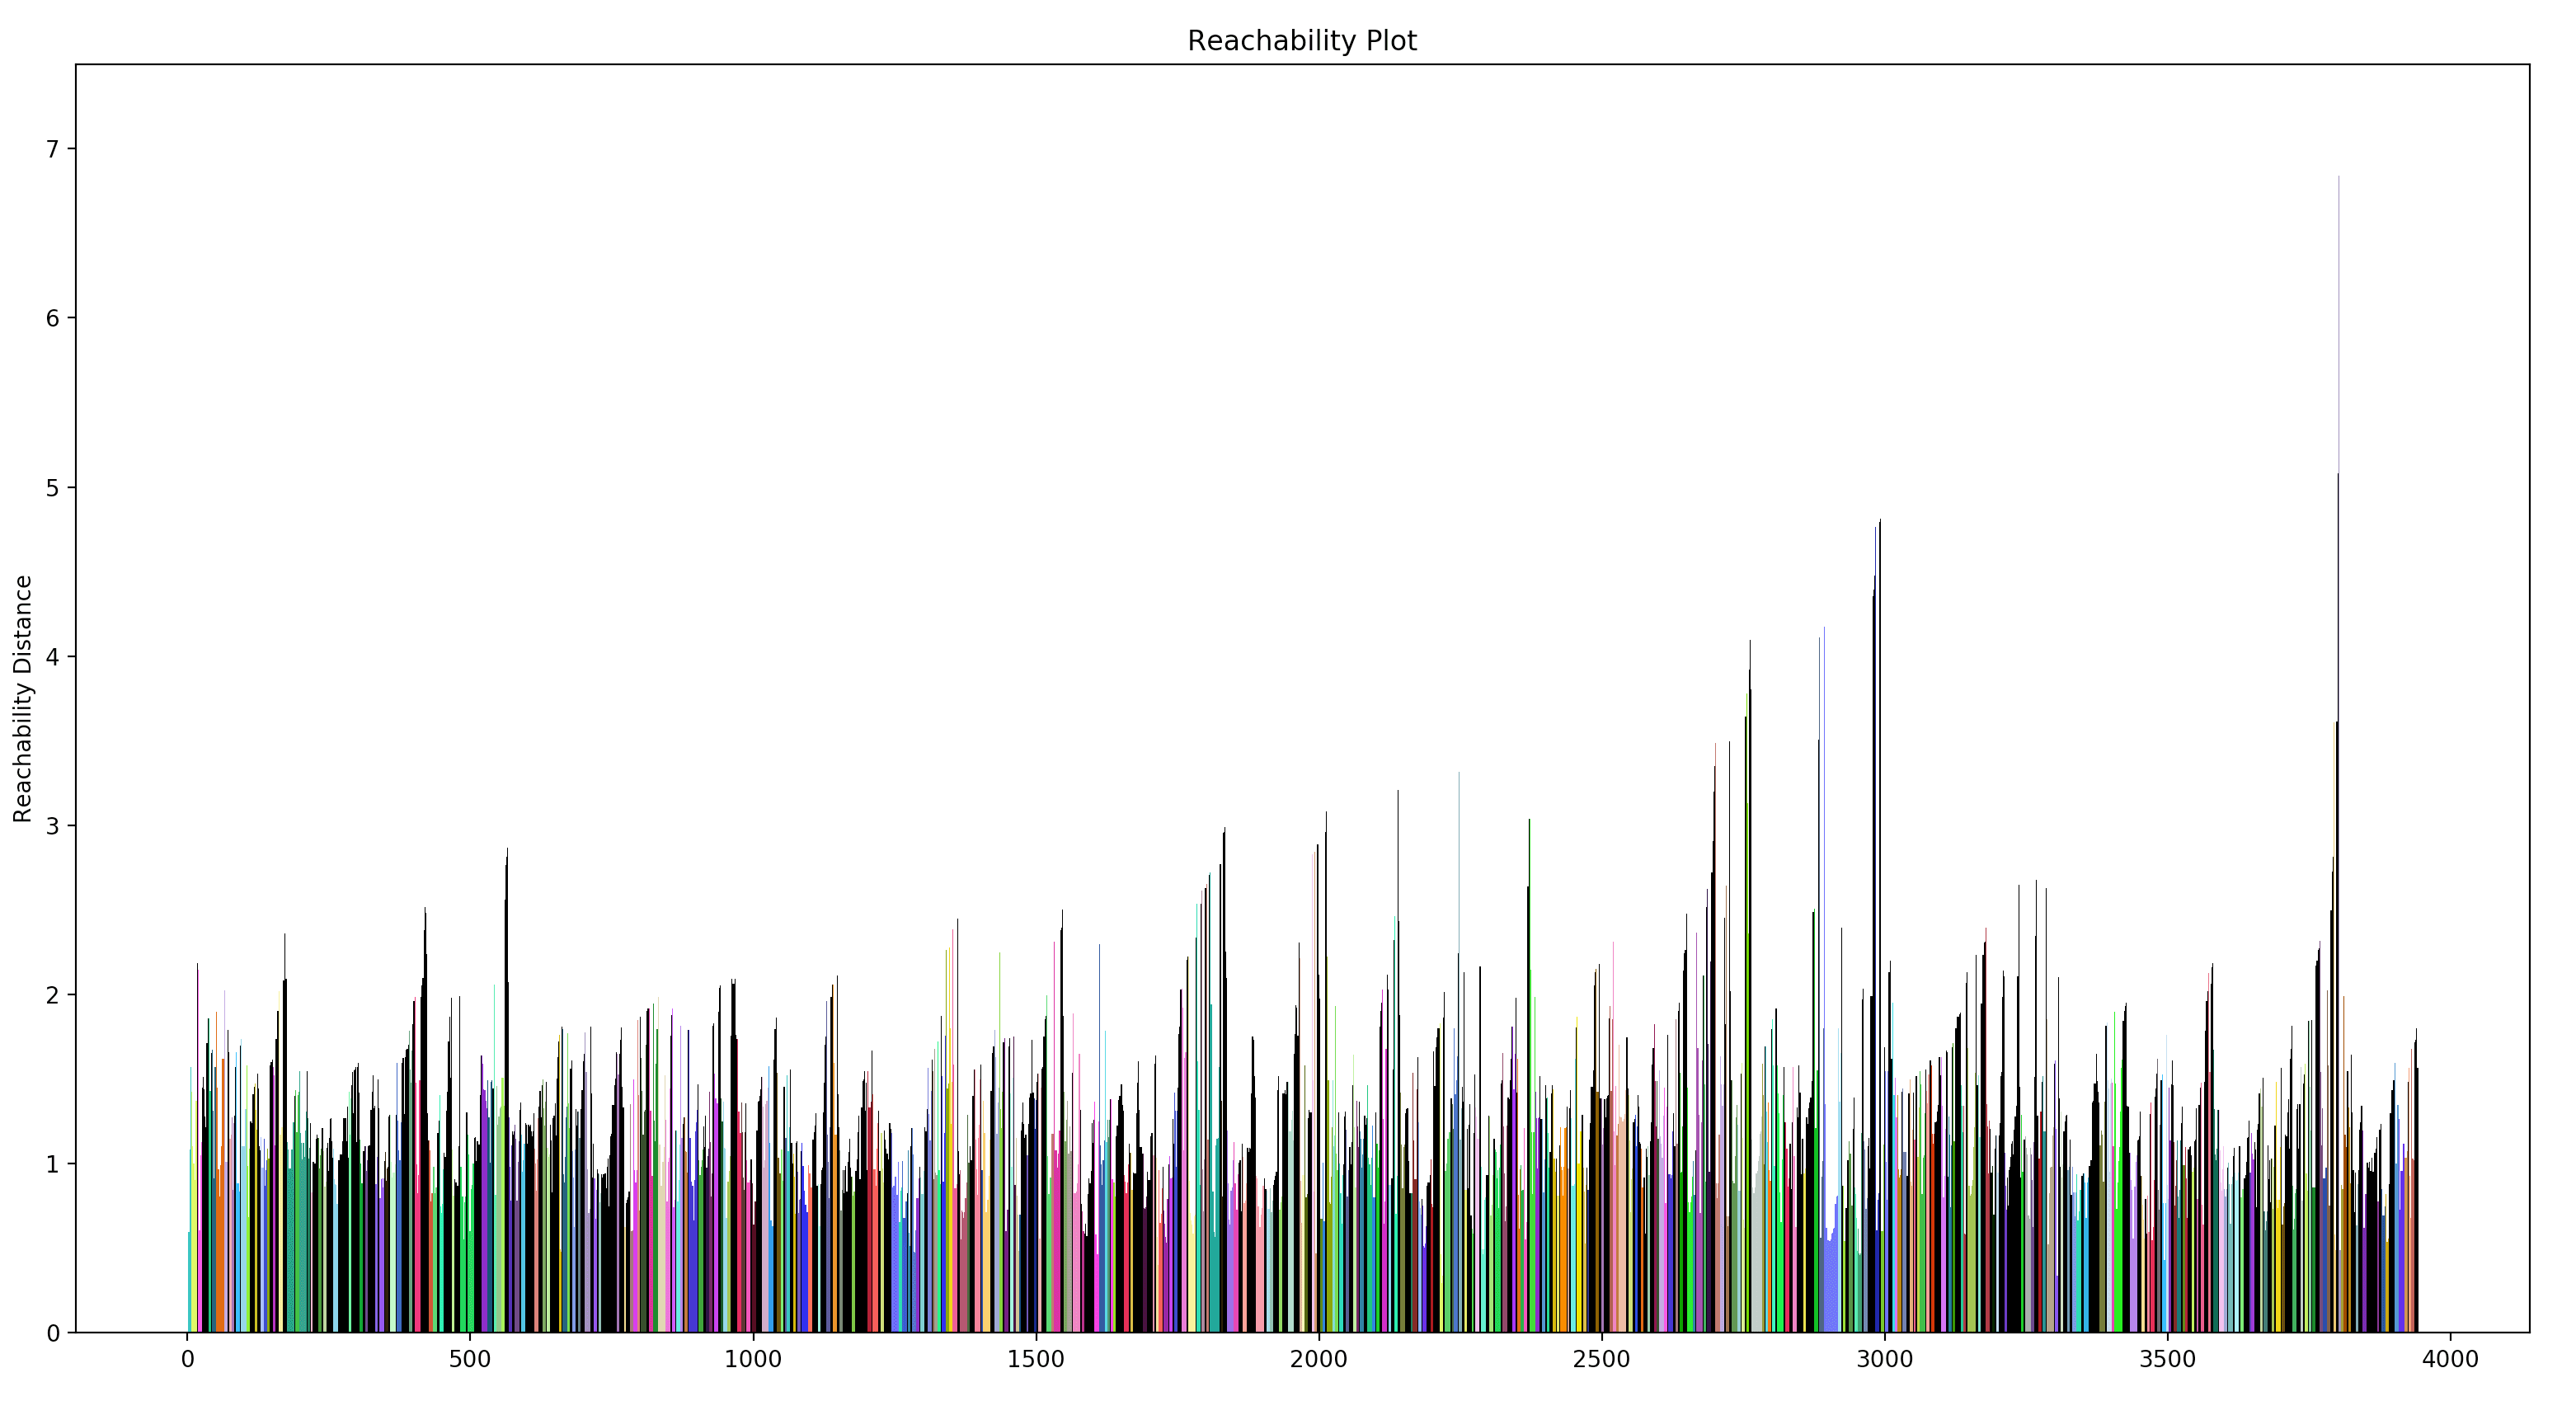
\includegraphics[width=1\textwidth]{./images/OPTICS/3h-1-reachabilityPlot-xi.png}
  \caption{\textbf{3h dataset} (first column - 30 min) OPTICS reachability plot using OPTICS automatic cluster extraction (\textbf{xi}). The coloured bars highlight clusters, whilst the black ones indicate noise.}
  \label{figure:fullSizeReachabilityPlotXi3h}
\end{figure}



\begin{figure}[H]
  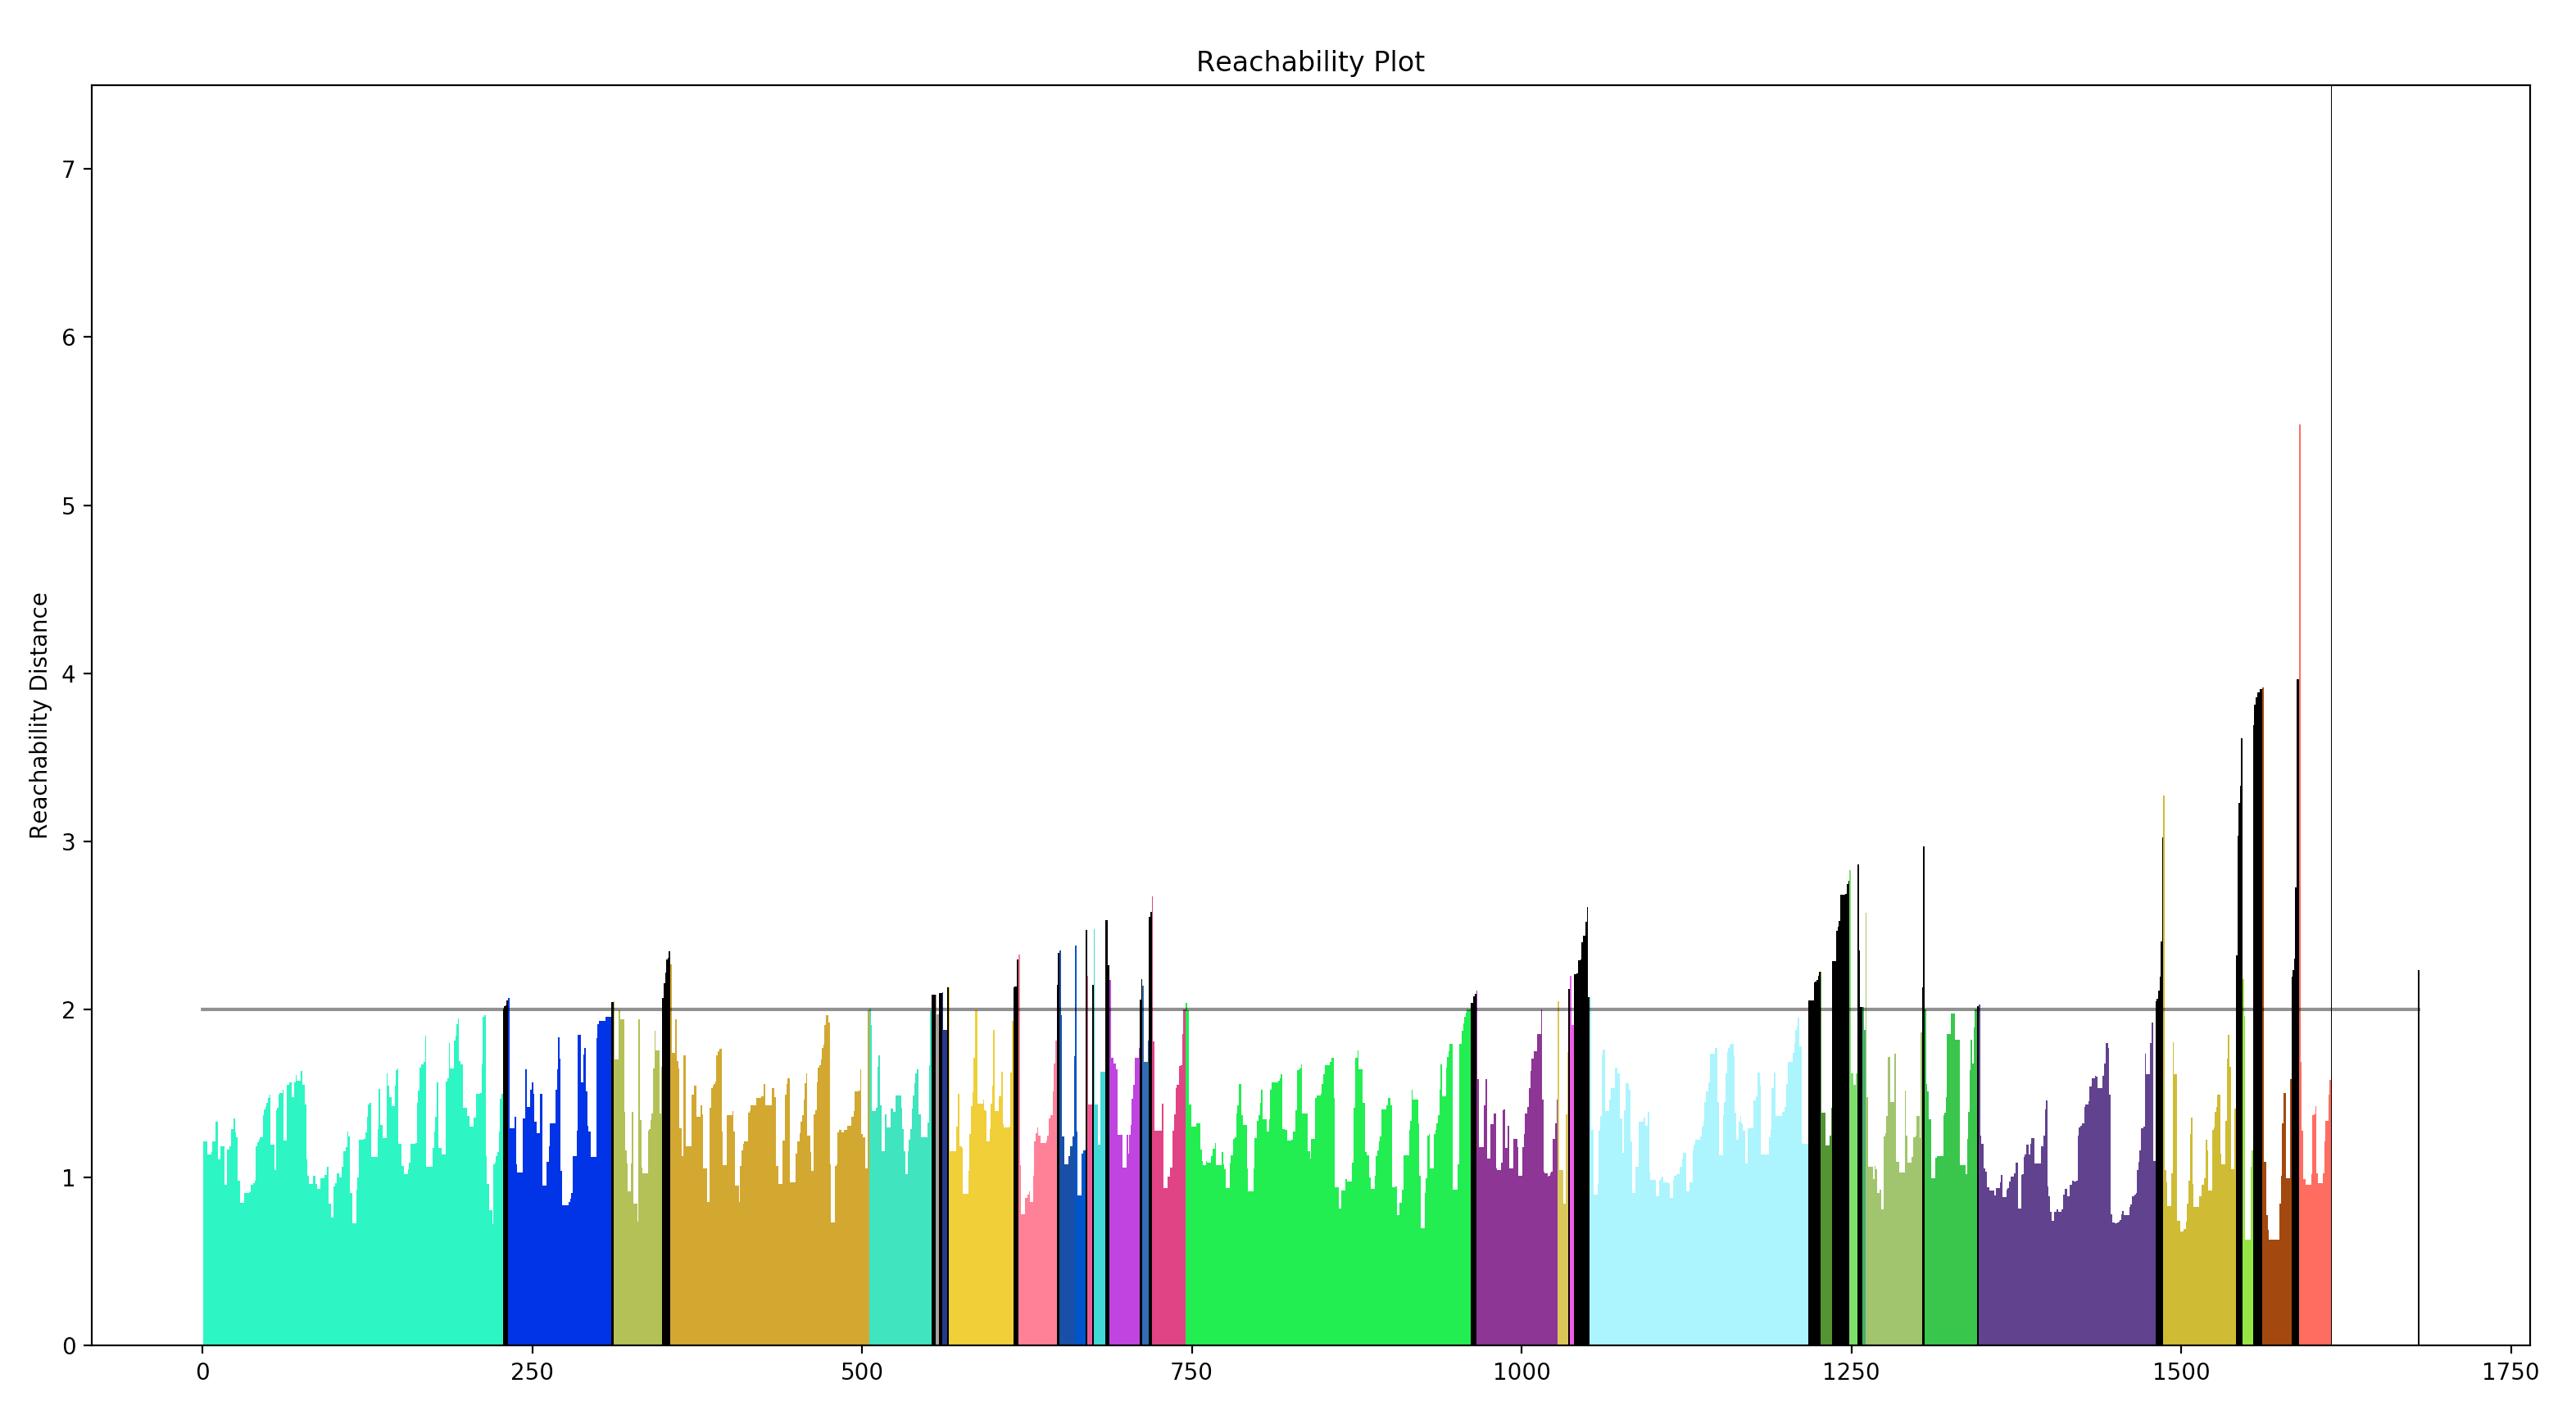
\includegraphics[width=1\textwidth]{./images/OPTICS/1h-1-reachabilityPlot-DBSCAN.png}
  \caption{\textbf{1h dataset} (first column - 15 min) OPTICS reachability plot using \textbf{DBSCAN} clustering. The coloured bars highlight clusters, whilst the black ones indicate noise. The eps parameter, set at 2, his highlighted with a horizontal line.}
  \label{figure:fullSizeReachabilityPlotDBSCAN1h}
\end{figure}

\begin{figure}[H]
  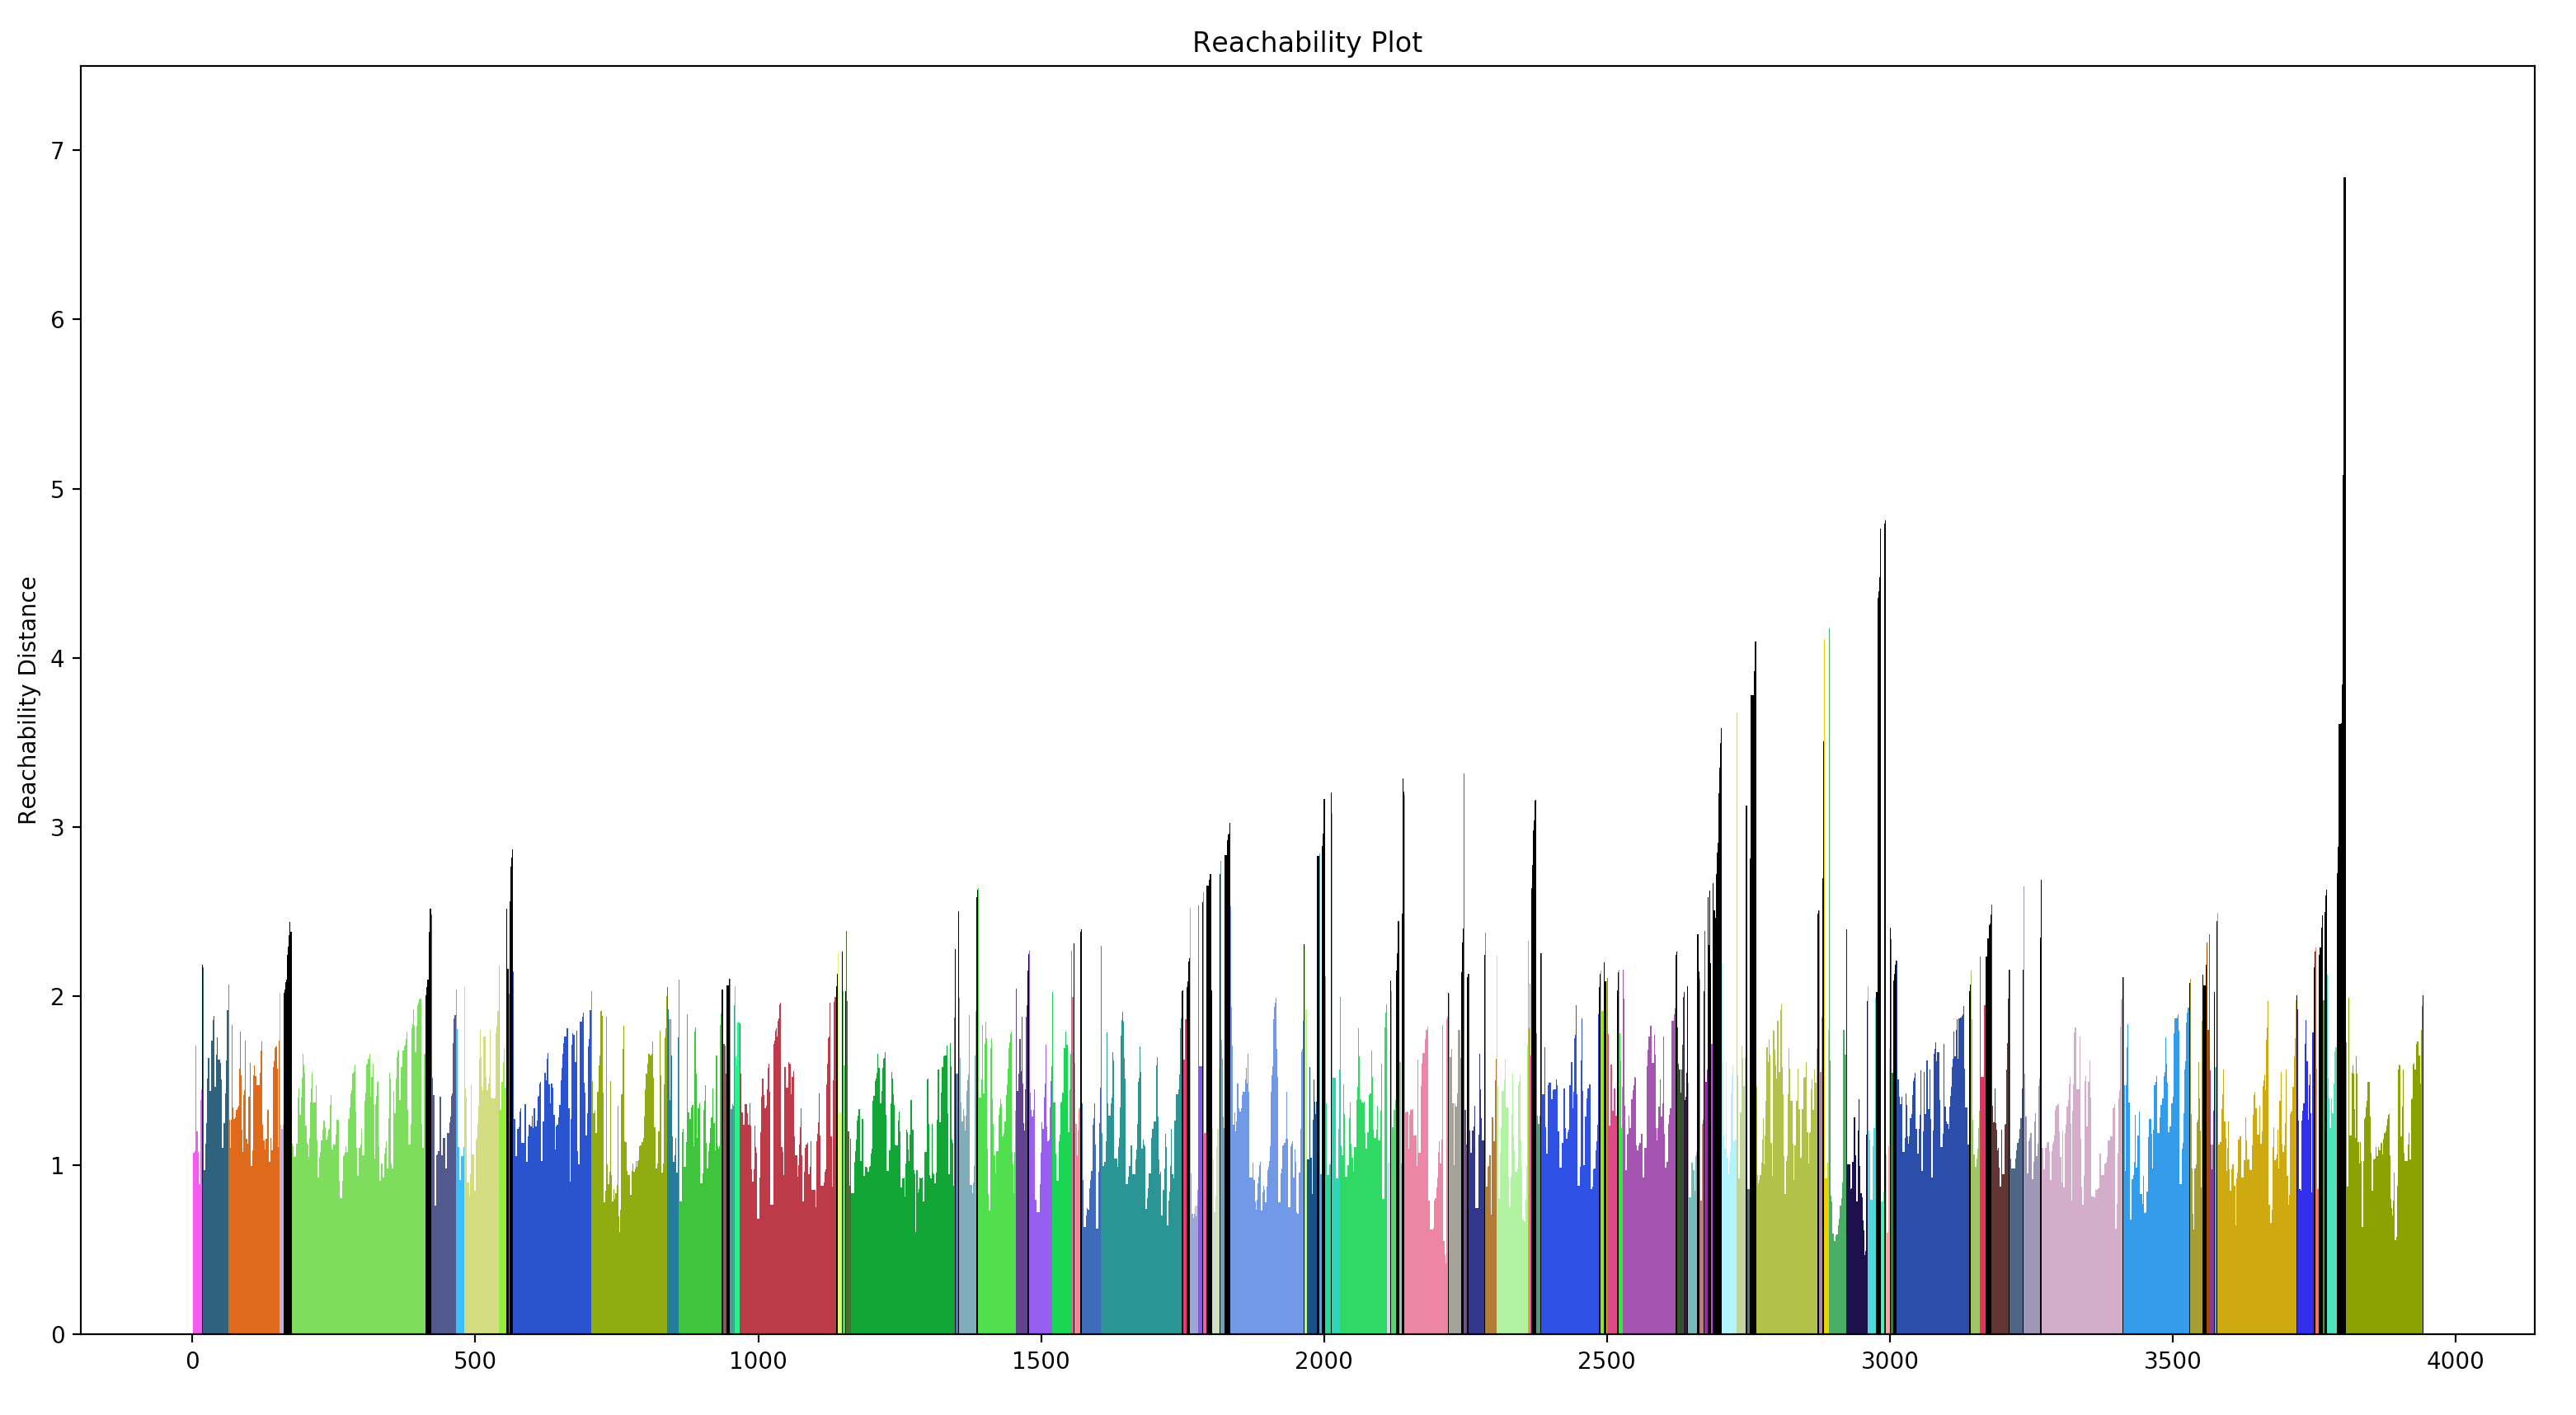
\includegraphics[width=1\textwidth]{./images/OPTICS/3h-1-reachabilityPlot-DBSCAN.png}
  \caption{\textbf{3h dataset} (first column - 30 min) OPTICS reachability plot using \textbf{DBSCAN} clustering. The coloured bars highlight clusters, whilst the black ones indicate noise. The eps parameter, set at 2, his highlighted with a horizontal line.}
  \label{figure:fullSizeReachabilityPlotDBSCAN3h}
\end{figure}




% \begin{figure}[H]
%   \centering
%   \begin{subfigure}{.5\textwidth}\captionsetup{width=.8\linewidth}
%     \centering
%     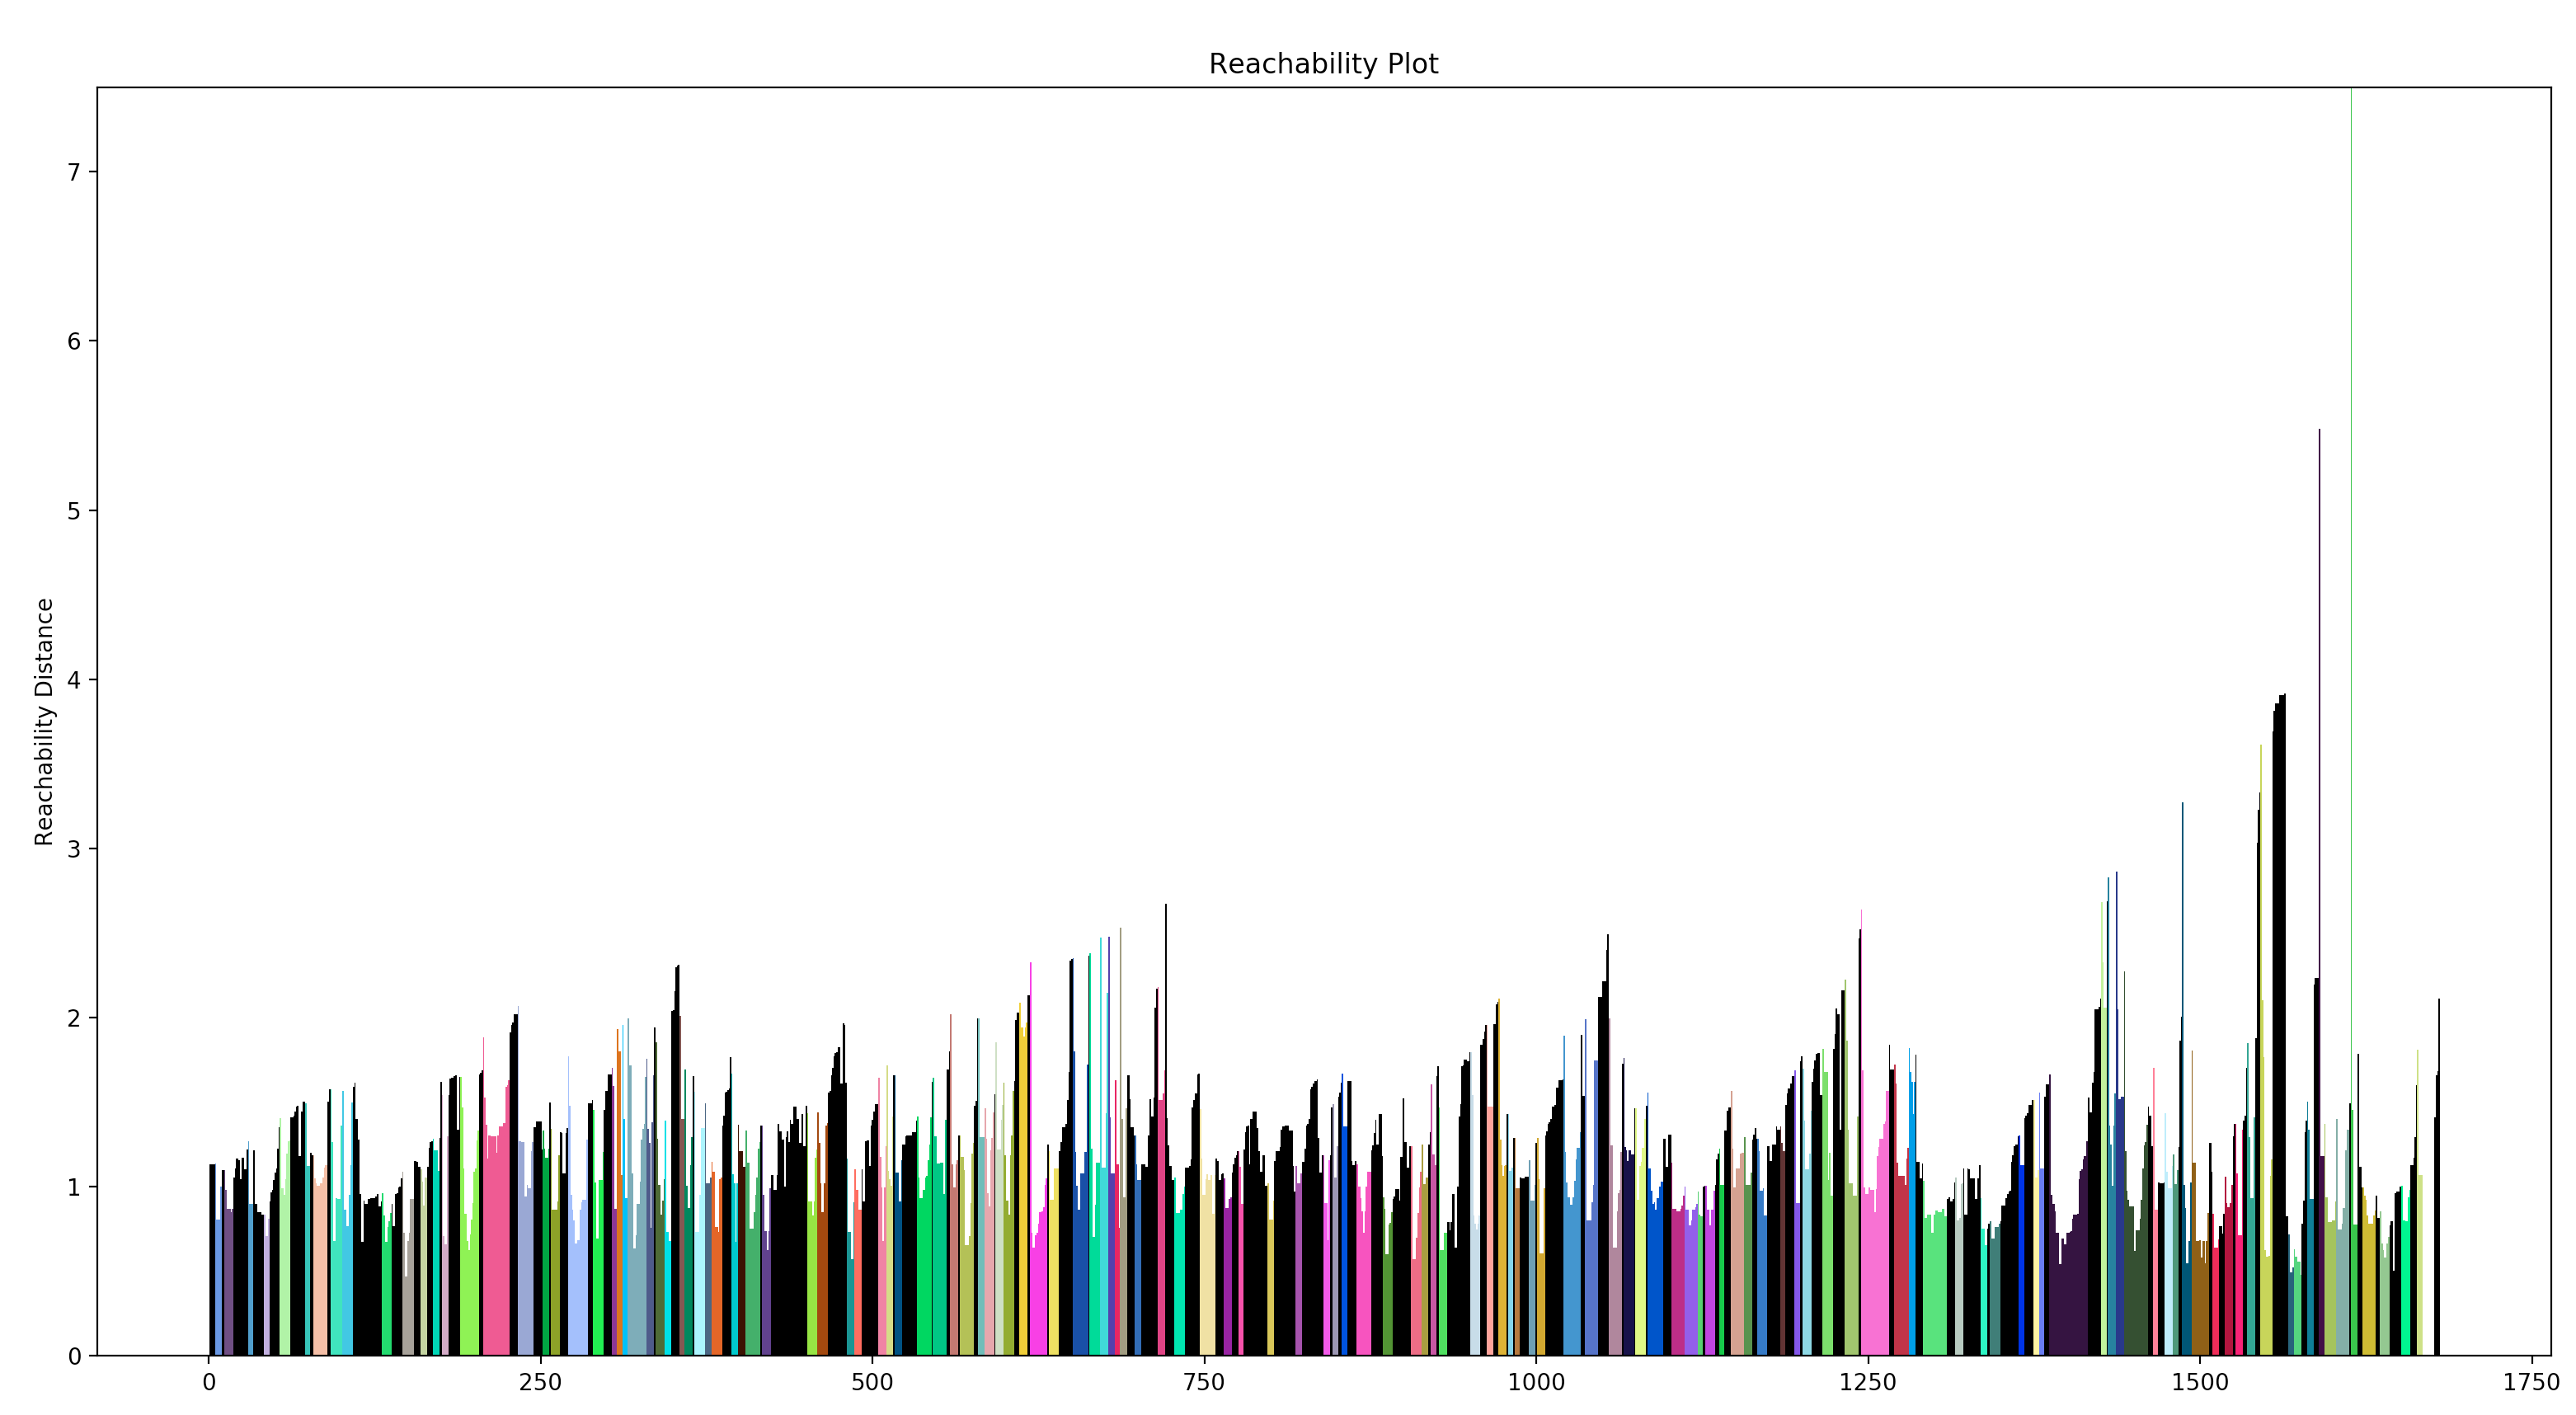
\includegraphics[width=1\textwidth]{./images/OPTICS/1h-1-reachabilityPlot-xi.png}
%   \caption{1h dataset (first column - 15 min)}
%   \end{subfigure}%
%   \begin{subfigure}{.5\textwidth}\captionsetup{width=.8\linewidth}
%     \centering
%     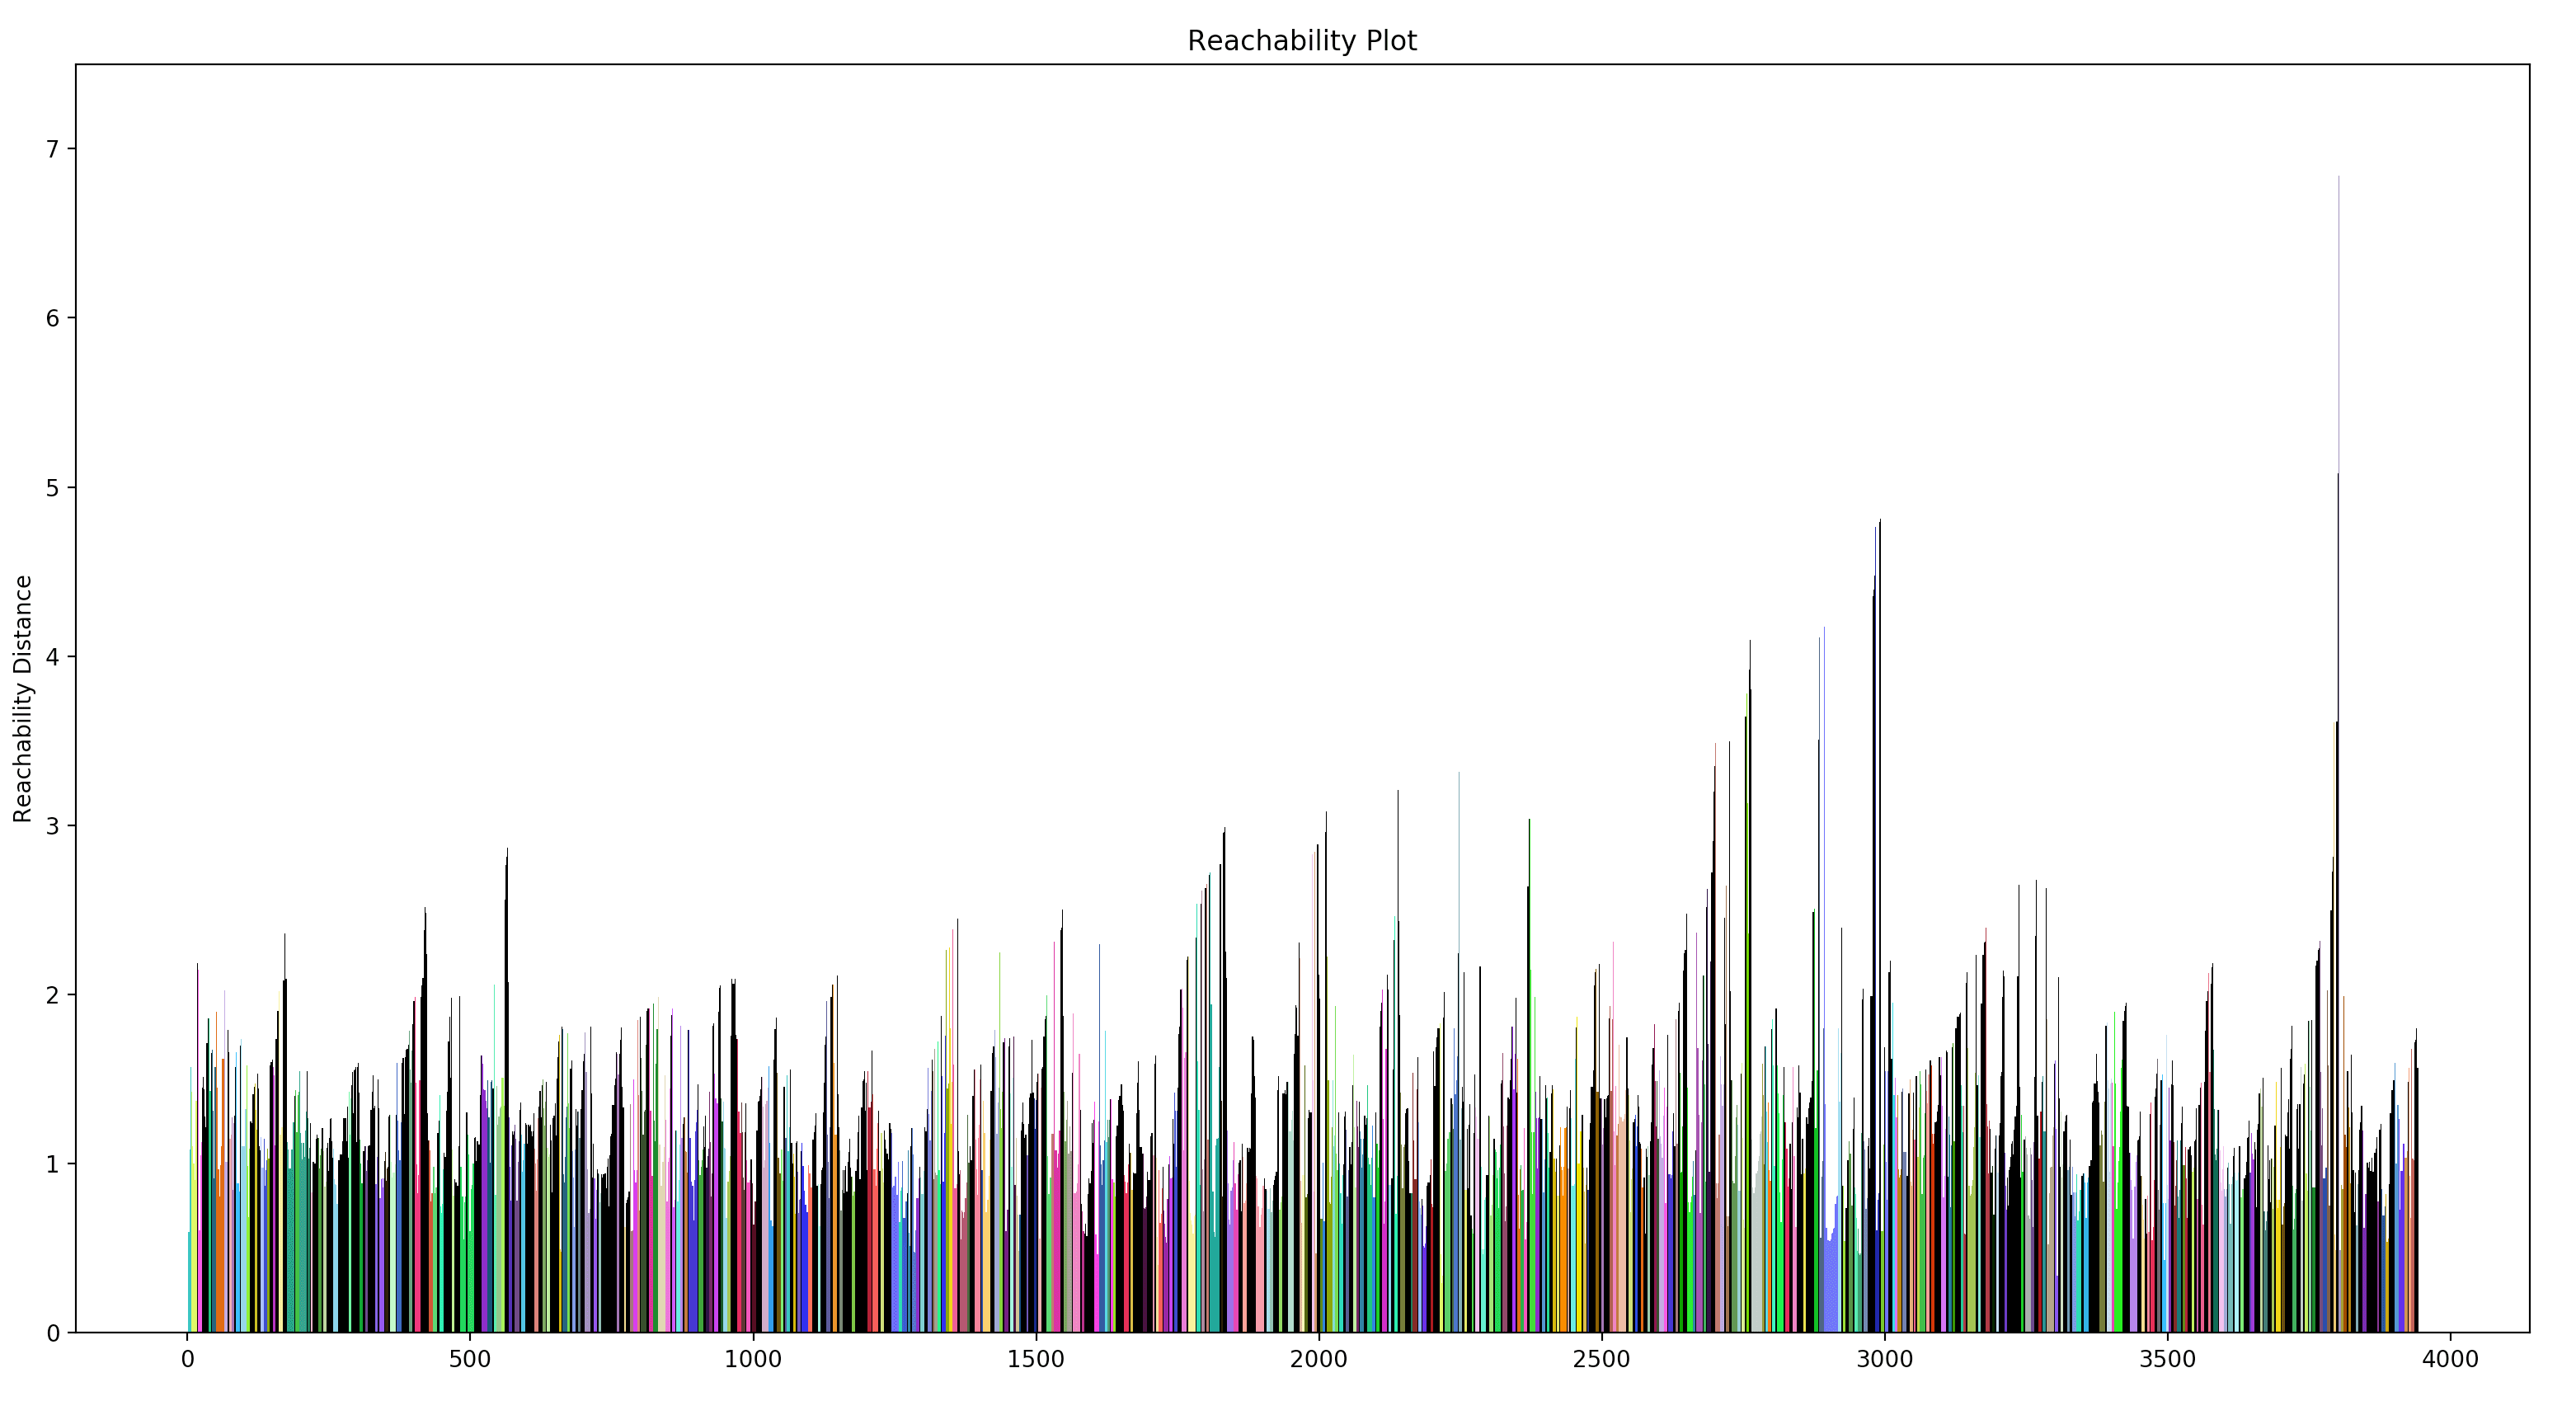
\includegraphics[width=1\textwidth]{./images/OPTICS/3h-1-reachabilityPlot-xi.png}
%     \caption{3h dataset (first column - 30 min)}
%   \end{subfigure}
%   \caption{OPTICS reachability plot using OPTICS automatic cluster extraction (xi). The coloured bars highlight clusters, whilst the black ones indicate noise.}
%   \label{figure:OPTICSXiResultsReachabilityPlot}
%   \end{figure}



% \begin{figure}[H]
%   \centering
%   \begin{subfigure}{.5\textwidth}\captionsetup{width=.8\linewidth}
%     \centering
%     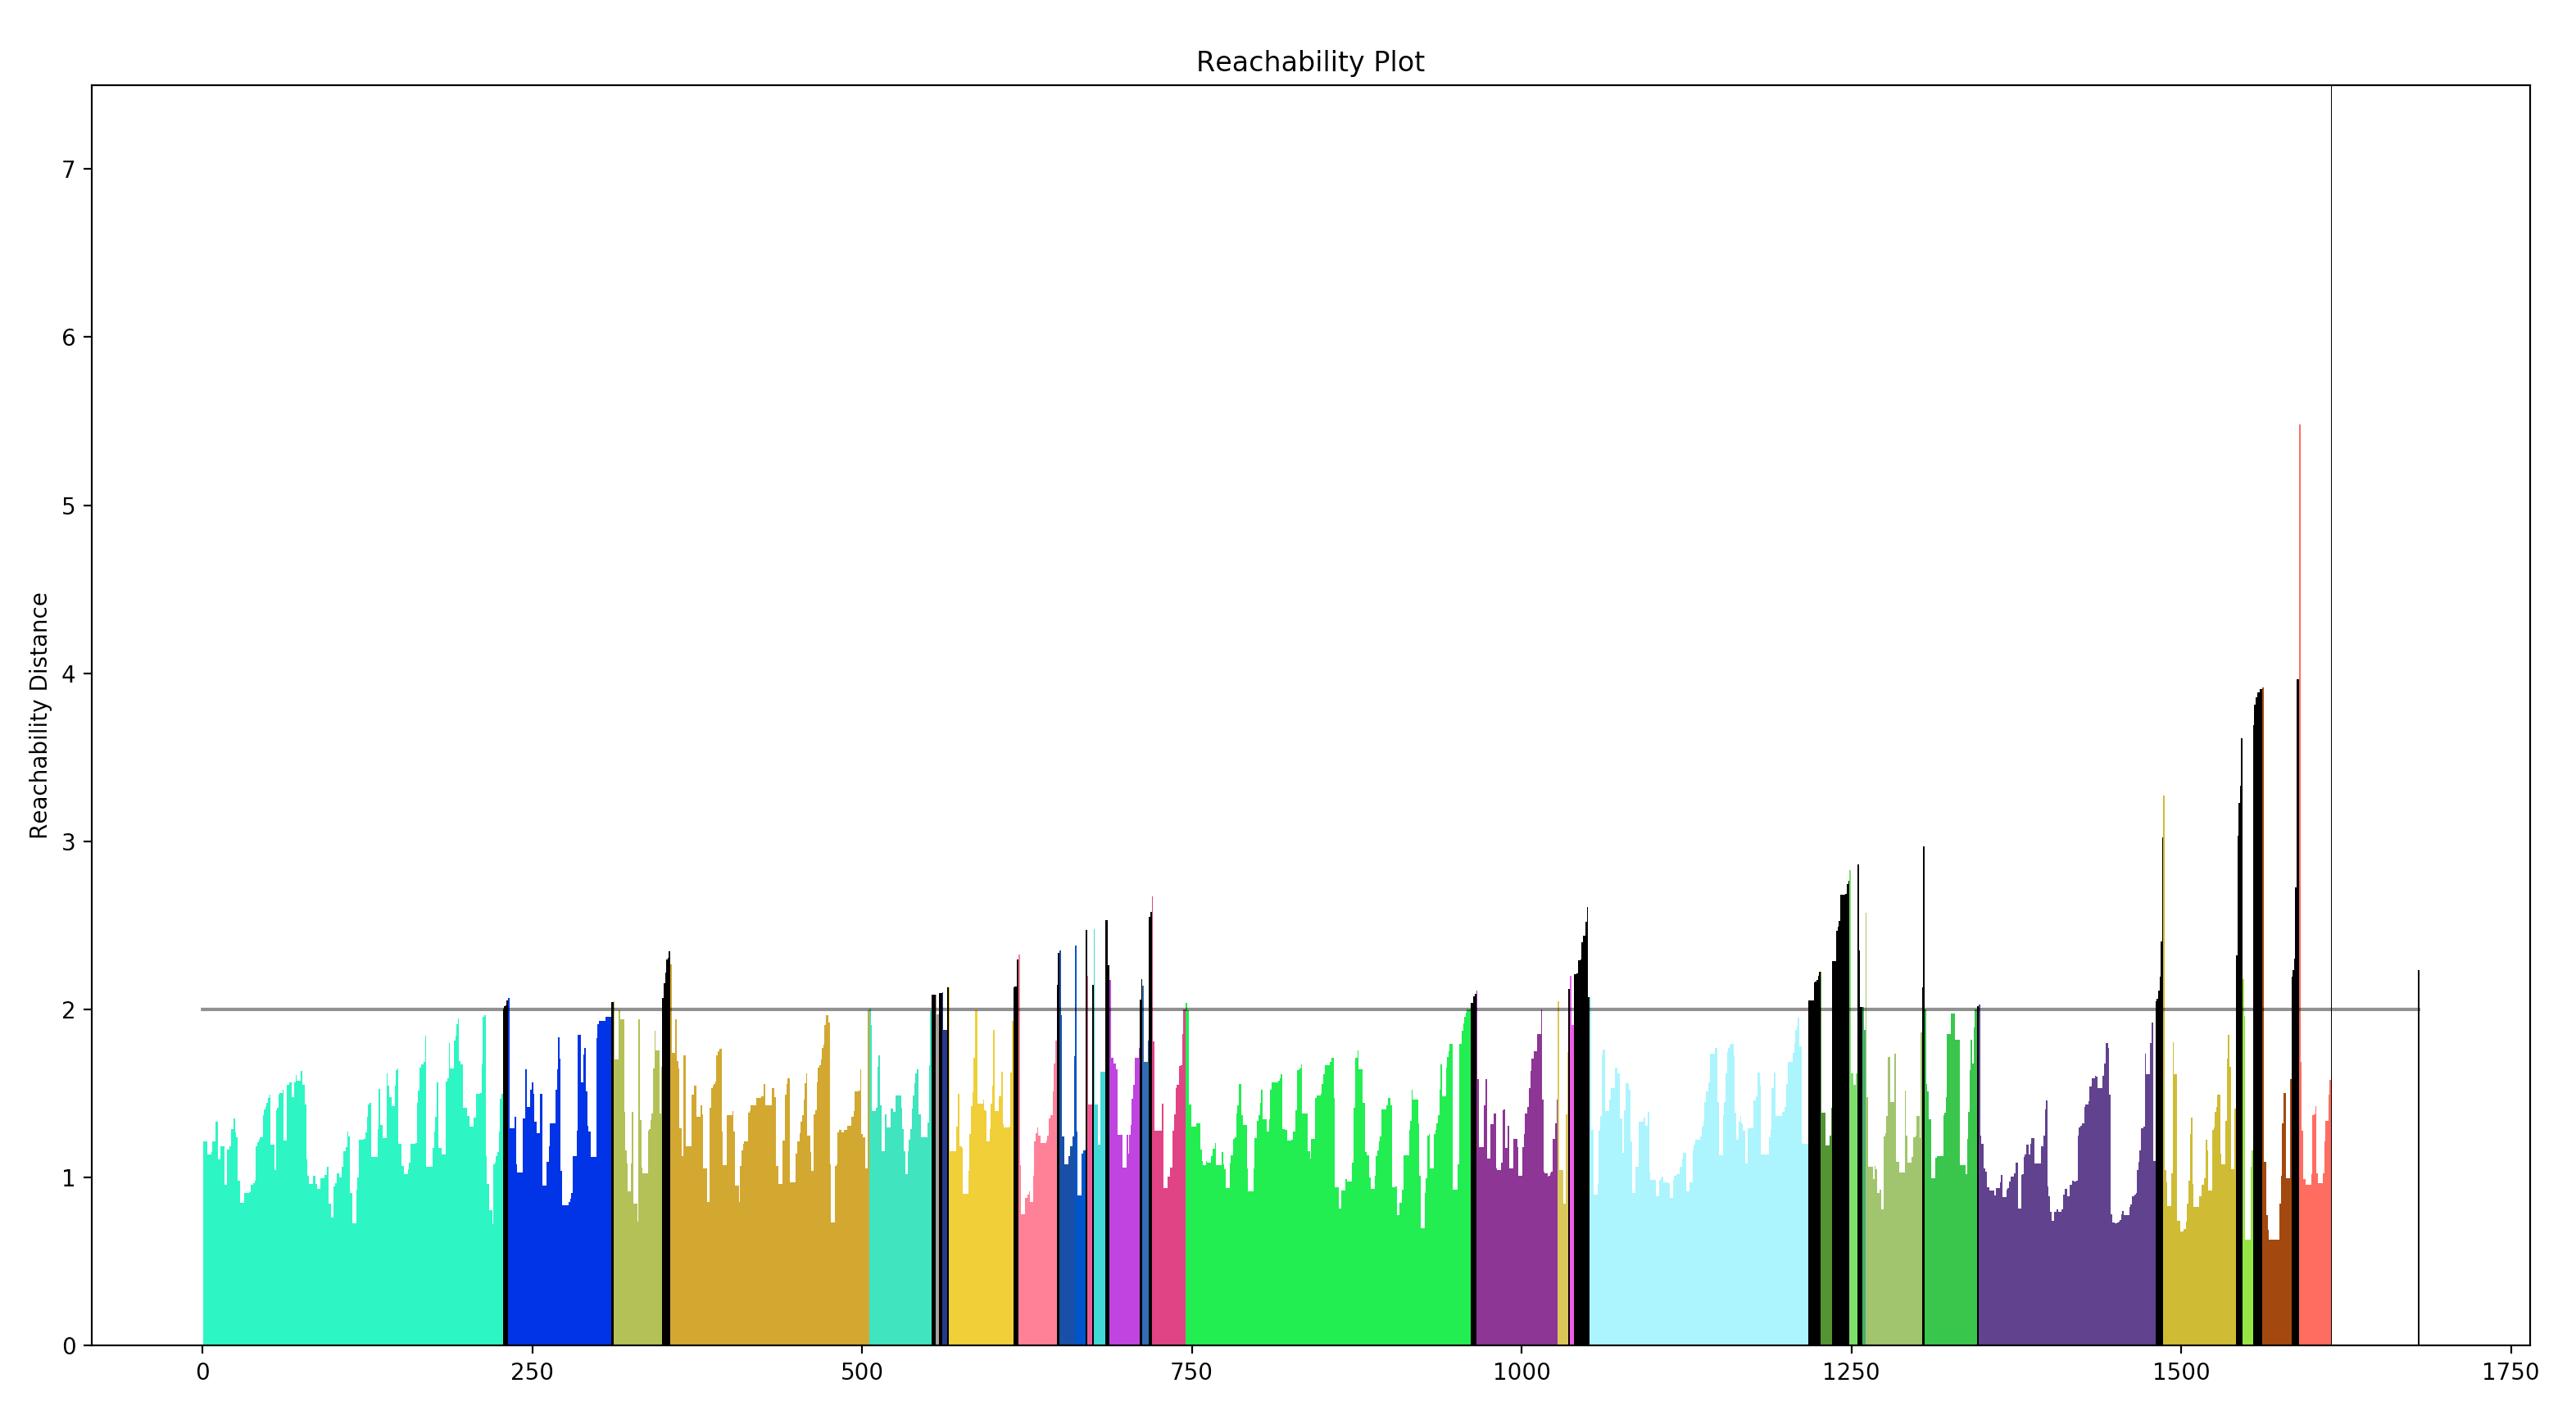
\includegraphics[width=1\textwidth]{./images/OPTICS/1h-1-reachabilityPlot-DBSCAN.png}
%   \caption{1h dataset (first column - 15 min)}
%   \end{subfigure}%
%   \hfill
%   \begin{subfigure}{.5\textwidth}\captionsetup{width=.8\linewidth}
%     \centering
%     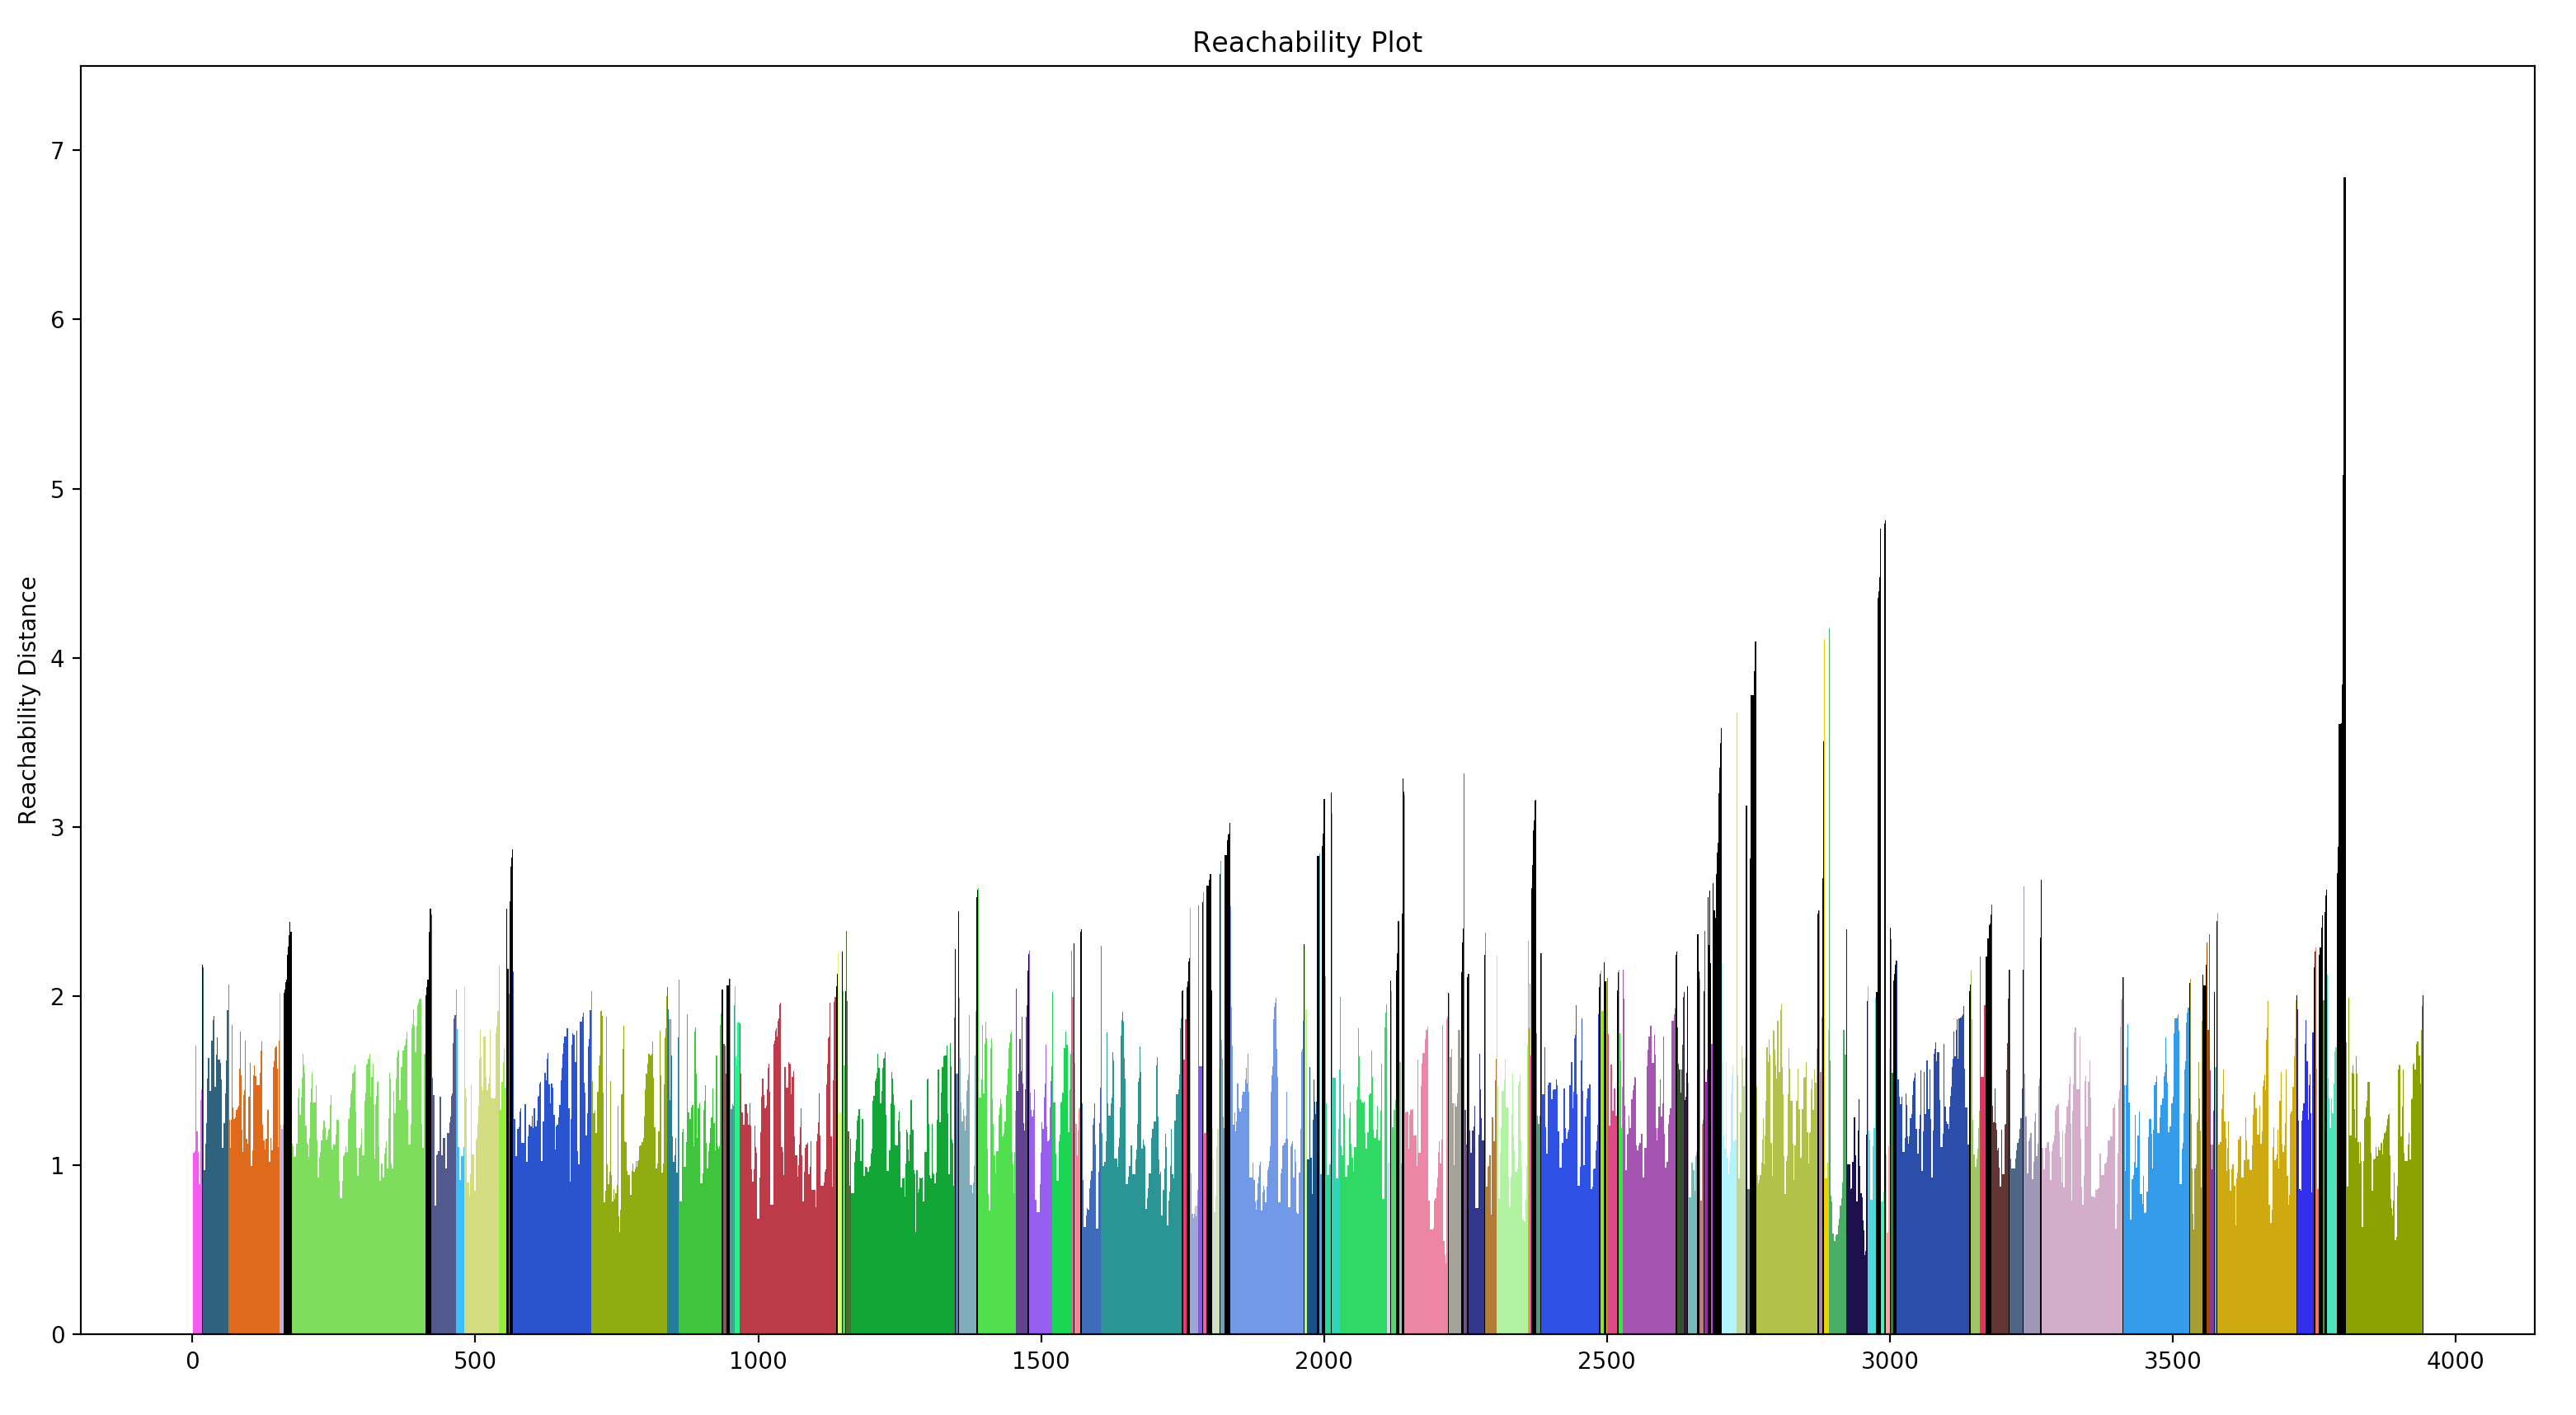
\includegraphics[width=1\textwidth]{./images/OPTICS/3h-1-reachabilityPlot-DBSCAN.png}
%     \caption{3h dataset (first column - 30 min)}
%   \end{subfigure}
%   \caption{OPTICS reachability plot using DBSCAN clustering. The coloured bars highlight clusters, whilst the black ones indicate noise. The eps parameter, set at 2, his highlighted with a horizontal line.}
%   \label{figure:OPTICSResultsReachabilityPlot}
%   \end{figure}
